\begin{figure*}
  \centering
 \includegraphics[width=.23\textwidth, height=4.5cm]{figures/p8.png} 
  \includegraphics[width=.2\textwidth, height=4.5cm]{figures/p1.jpg} 
    \includegraphics[width=.18\textwidth, height=4.5cm]{figures/p6.png} 
    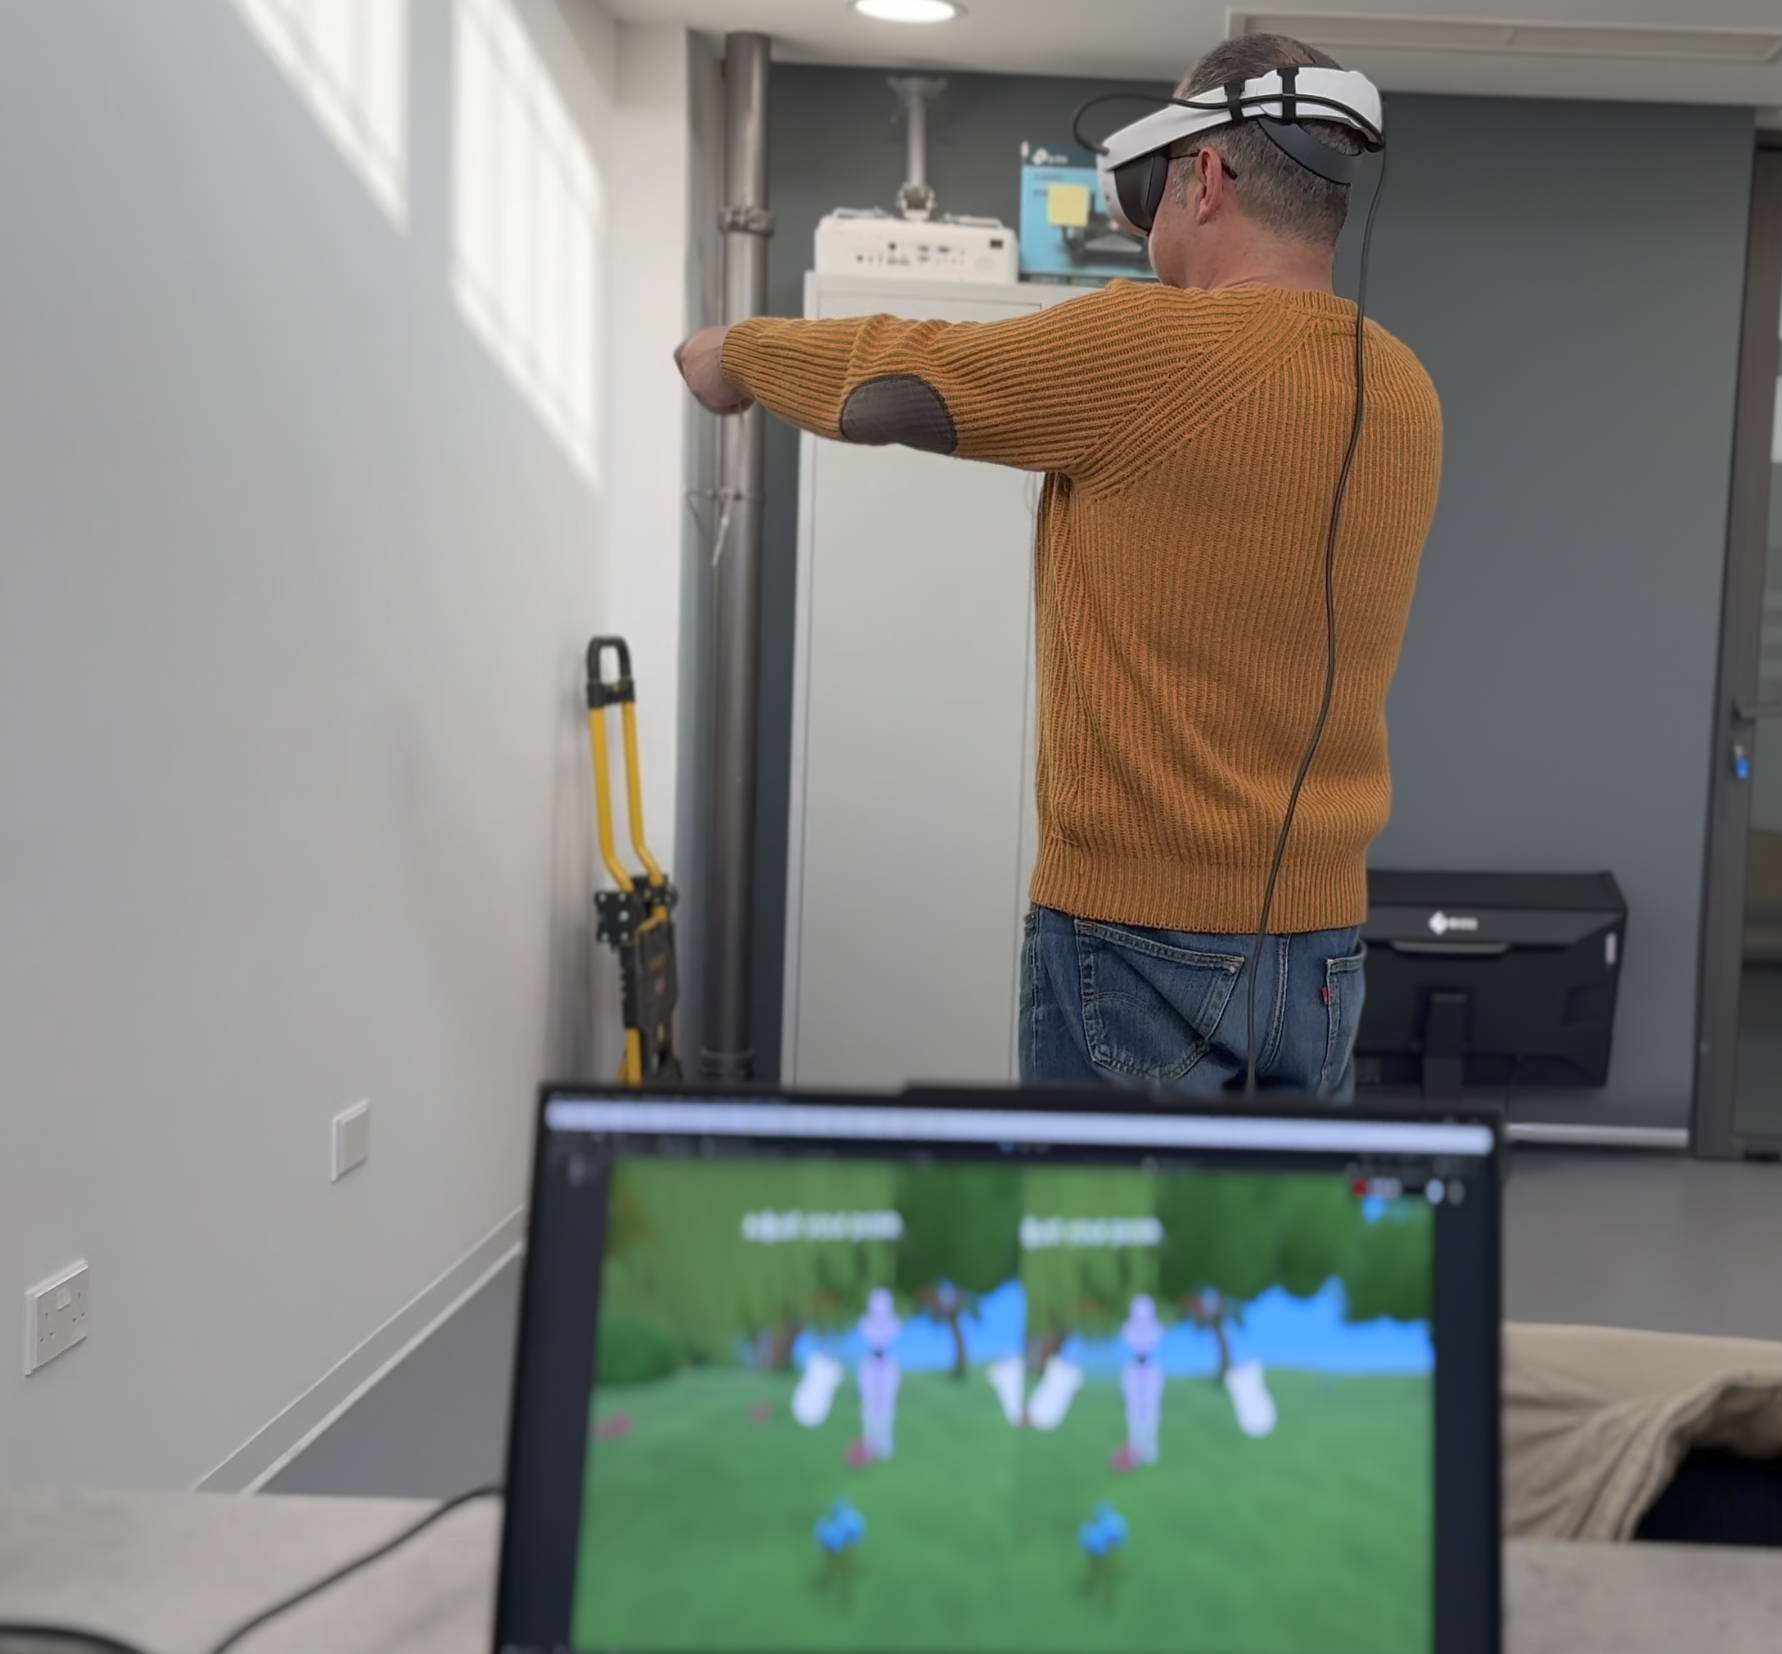
\includegraphics[width=.28\textwidth, height=4.5cm]{figures/p9.png} 
      

\caption{Participants using Tranquil Loom during the workplace deployment. The in-situ deployment allowed us to observe how participants engaged in well-being activities in a realistic work context.}  
\label{fig:participants}

\end{figure*}

\section{Tranquil Loom}
\label{sec:app}


Based on the six design requirements identified in our formative study, we developed \textit{Tranquil Loom} (Figure \ref{fig:interaction}). It is a prototype VR well-being app designed to support short and restorative breaks during the workday. The app offers three types of well-being activities: stretching, guided meditation, and free exploration in four environments addressing DR1 (supporting a range of well-being needs) and DR2 (structured and unstructured activity options).

\smallskip
\noindent\textbf{Platform and Implementation.} Tranquil Loom was developed in Unity (version 6000.0.23f1) and deployed on the Meta Quest 3 using Meta Quest Link for PC streaming. Interaction was handled through Unity’s XR Interaction Toolkit and the Meta XR SDK.
\smallskip

\smallskip
\noindent\textbf{Environments.} The app includes four environments: forest, snowy landscape, beach, and an abstract space; these were assembled from Unity asset store models (Figure \ref{fig:teaser}). The environments had a stylized aesthetic as per the results of our formative study, and were selected based on participant preferences for both natural settings and more abstract and minimalist spaces. Each environment includes subtle animated elements (e.g., swaying trees, drifting snow). Users can perform any activity in any environment; this supports both our DR4 (diversity of environments) and DR5 (multipurpose use). We avoided overly realistic environments because creating highly detailed assets would have increased the risk of performance issues or motion sickness, while using 360 videos rather than 3D worlds would not have allowed for introducing the exploration mode and possibly reduce feelings of immersion \cite{ppali_keep_2022}.


\smallskip
\noindent\textbf{Sound Design.} All environments include spatialized nature sounds (e.g., water, wind, or bird songs). The abstract and home environments feature ambient music generated using \url{suno.ai}. The meditation activity includes a voice track (guided session) created using \url{elevenlabs.io}; this supports our DR1 (supporting a range of well-being needs) and DR3 (short, focused sessions). 

\smallskip
\noindent\textbf{User Journey and Personalization.} Upon launching the app, users begin in a calming home scene with two interactive panels. At the top of the first panel, a virtual agent named Loomi invites reflection with the prompt: ``What's weighing on you recently?''. Users can select from six preset feelings (i.e., mentally drained, restless, lacking motivation, overwhelmed, stiff or tense, need a reset), which were derived from our interview data and literature on workplace stress and emotional check-ins \cite{wagener_role_2021}. Based on the selected response, Loomi replies with a short message acknowledging the feeling and offers two suitable activity–environment suggestions. The interaction structure follows therapeutic communication strategies, that is, acknowledge, normalize, and recommend. These strategies are commonly used in mental health and counseling contexts \cite{cuff_empathy_2016}. Loomi's replies are generated using a large language model (LLM) via the OpenAI GPT-4o API, tailored through a prompt\footnote{\url{https://github.com/EX-MRG-CYENS-CoE/healthXR/}} that limits its behavior to a supportive and empathetic tone. While Loomi does not rely on open-ended natural language input, integrating an LLM enables lightweight personalization and context-sensitive recommendations in a conversational format. This feature supports DR6 (personalized and context-aware recommendations) and serves as a proof-of-concept for embedding LLM-driven agents within VR well-being apps~\cite{fang2024practicing}. We deliberately opted for multiple-choice input to minimize cognitive load and avoid typing-related frustration \cite{bhatia_text_2025}. However, this choice may have limited the depth of personalization we were able to introduce.
\smallskip


\noindent\textbf{Activities.} Tranquil Loom includes three activity modes: stretching, breathing, and open-ended exploration. To address DR4 (diversity of environments) and DR5 (multipurpose environments), the app allows users to choose one of three activities in any of four environments. Users can also end a session at any time and start a new one with a different activity or environment. This supports flexibility while keeping sessions short and focused as per DR3.
\smallskip

\noindent\emph{Stretching.} In the stretching mode, users follow a humanoid avatar demonstrating a sequence of six office-friendly stretches. These are primarily upper-body movements that avoid the need for floor-based poses or clothing changes, supporting DR3 (low-effort engagement). The app uses inverse kinematics to estimate the user’s body pose from head and hand positions. Above the avatar's hands, color-changing indicators (red to green) provide feedback on the correct form. Once alignment is achieved, a timer starts; if the user breaks form, it resets. The app includes three difficulty settings: bliss (10s), harmony (15s), and zen (30s). These were adapted from posture and movement guidance literature \cite{page_current_2012}. We chose not to include users' full-body representation. Instead, only the user's hands and guide avatar are visible. This choice allowed us to ensure the user's focus remained on mirroring the stretching poses.
\smallskip

\noindent\emph{Meditation.} In the meditation mode, the user's journey begins with a 2-minute voice-guided breathing session. The script is designed to support short, focused interventions during the workday, aligning with evidence that even brief meditation sessions can reduce stress and support cognitive clarity in knowledge workers \cite{zeidan_mindfulness_2010}.
\smallskip

\noindent\emph{Exploration.} In the exploration mode, users can freely navigate the environment using joystick movement. We considered implementing teleportation (common for reducing motion sickness), but ultimately chose joystick movement to support precise navigation and movement continuity \cite{buttussi_locomotion_2021}. To reduce discomfort, we limited movement speed and designed all environments as open spaces with minimal visual clutter. The ability to simply ``be'' in a space and explore it without a specific task supports DR2 (unstructured activity) and DR4 (emotional fit with the environment).
\smallskip








% \textbf{The Stretching System in the well-being VR App provides guided posture correction using Inverse Kinematics (IK) and real-time movement analysis. The system tracks the user's head, hands, and body positioning using the Oculus Quest 3’s hand-tracking and controller input. A two-bone IK solver is implemented to correct arm movements and ensure accurate stretching poses. The system employs the FABRIK (Forward And Backward Reaching Inverse Kinematics) algorithm, which iteratively adjusts joint positions to match an ideal target posture:}

% \[
% p_i = p_{i-1} + d_i \frac{(p_{i+1} - p_i)}{\lVert p_{i+1} - p_i \rVert}
% \]

% \textbf{where $p_i$ represents the position of the i-th joint, and $d_i$ is the segment length. The stretching system also calculates an alignment score by comparing the user’s pose with predefined reference postures, using cosine similarity for joint angle validation:}

% \[
% S = \frac{\sum\limits_{i=1}^{n} \theta_i \cdot \theta_i^{ref}}
% {\sqrt{\sum\limits_{i=1}^{n} \theta_i^2} \cdot \sqrt{\sum\limits_{i=1}^{n} (\theta_i^{ref})^2}}
% \]

% \textbf{where $\theta_i$ represents the user’s joint angles and $\theta_i^{ref}$
% represents the ideal reference angles. If the similarity score falls below a threshold, the system provides real-time visual and auditory feedback to guide the user toward correct alignment.}



% \noindent\textbf{Additional Features}
% Users can navigate between environments and activities via a simple menu that opens with the X button. This menu also allows users to adjust audio volume and enable or disable vibration feedback during stretching sessions. The Home screen also includes two non-functional panels for illustrative purposes: a) A leaderboard, suggesting potential for light gamification or social use, b) A GDPR statement, signaling awareness of privacy and data protection, even though no personal data was collected during the study The features were included to provoke thought about possible extensions of such a tool in future workplace settings.
% \textbf{User Journey and functionality.} When the user enters the app they are welcomed on a Home scene featuring two panels. On the top of the first panel the user is welcomed by a virtual guide called lumi and they  asked What is on your mind recently? And they have 6 options to respond  from (overwhelmed, tired, restless, demotivated, stiff or tense, stressed). the options were generated based on what people told us they feel during the interviews but also just as placeholders to get people to think about what has been troubling them recently. We added this feature based on X's work who told about the importance of VR applications for mental health to prompt emotional reflection. We added pre-defined options to avoid the bothersome of having to type. When the user select then Loomi responds to them. First she acknowledge the user's challenge in one sentence, validate their experience so they feel heard. Then in one sentence they normalise their experience, letting them know this is a common issue for knowledge workers. Then Lumi  recommend two environment-functionality pairings, Suggesting two options that align with their challenge. This is dne based on X guidelines from psychotherapy. Loomi in the back end uses Open AI's API and we gave a prompt for the chatbot to respond this way. We added this feature here to showcase in a lightway the potential of Using AI in such applications. Below the Loomi panel there is the 4 environment options (Forest, Snow, Beach, Abstract) When the user clicks on an environment they are able to choose between 3 activities: Stretching, Meditation and Exploration. The Stretching activity features an avatar showcasing the user the pose they need to keep with their body. Above each of the hands of avatar there is the words left and right.  By tracking the position of the controlers we know if the user is in the correct position. If they are far from the position the words are red. The nearer they are to the position the words turn more green, turning fully green when they have reached the position. Then a timer starts. if they break position the timer restarts. if they keep the position for the asigned time then they get a message position completed and the pose changes. We have 6 poses in total. all quite simple and based on light arm stretches. We also have 3 modes of difficulty, each mode asking the user to keep the position for more or less seconds. In the exploration mode, the user is free to move around the environments and explore them freely using the joystick. The environments are intentionally large for this purpose. We didn't use teleportation as with the hoystick movement feels more relaistic but also users are able to determine exactly where they want to go. In the meditation session users enter the environment welcomed by the voice of Loomy who then eases them in to a 2 muinte guided breathing session. Users are able to navigate between environments through a menu that pops up when they push the X button. in this menu they can also adjust sound volume and turn on or off vibration feedback for stretching.  In the home screen we also have panels showcasing A LEADERship board and a GDPR statement. these doesn't actually work but are there to indicate the potential of such features such as a social component and the possibility of collecting personal data for feedback meaning that users need to be aware of their rights. 